\documentclass{article}

% Language setting
% Replace `english' with e.g. `spanish' to change the document language
\usepackage[french]{babel}
\usepackage[fleqn]{amsmath} % Aligner les équations à gauche


% Set page size and margins
% Replace `letterpaper' with`a4paper' for UK/EU standard size
\usepackage[letterpaper,top=2cm,bottom=2cm,left=3cm,right=3cm,marginparwidth=1.75cm]{geometry}

% Useful packages

\usepackage{amsmath}
\usepackage{graphicx}
\usepackage{subcaption}
\usepackage[colorlinks=true, allcolors=blue]{hyperref}

\title{TD 6 - Dipôle électrostatique}
\author{IPESUP - PC }
\date{16/10/2024}

\begin{document}
\maketitle

\section{Rappels de cours}

\textbf{Définition: }

Un dipôle électrostatique est un ensemble de deux charges opposées $-q$ et $+q$ assimilées à des charges ponctuelles. On étudie leurs effets à des distances grandes devant la distance qui les sépare. \\

Le \textbf{moment dipolaire} est le vecteur $\vec{p} = q \vec{NP}. $ Attention, $N$ est le point de la charge négative et $P$ celui de la charge positive.

\begin{figure}[h]
  \centering
  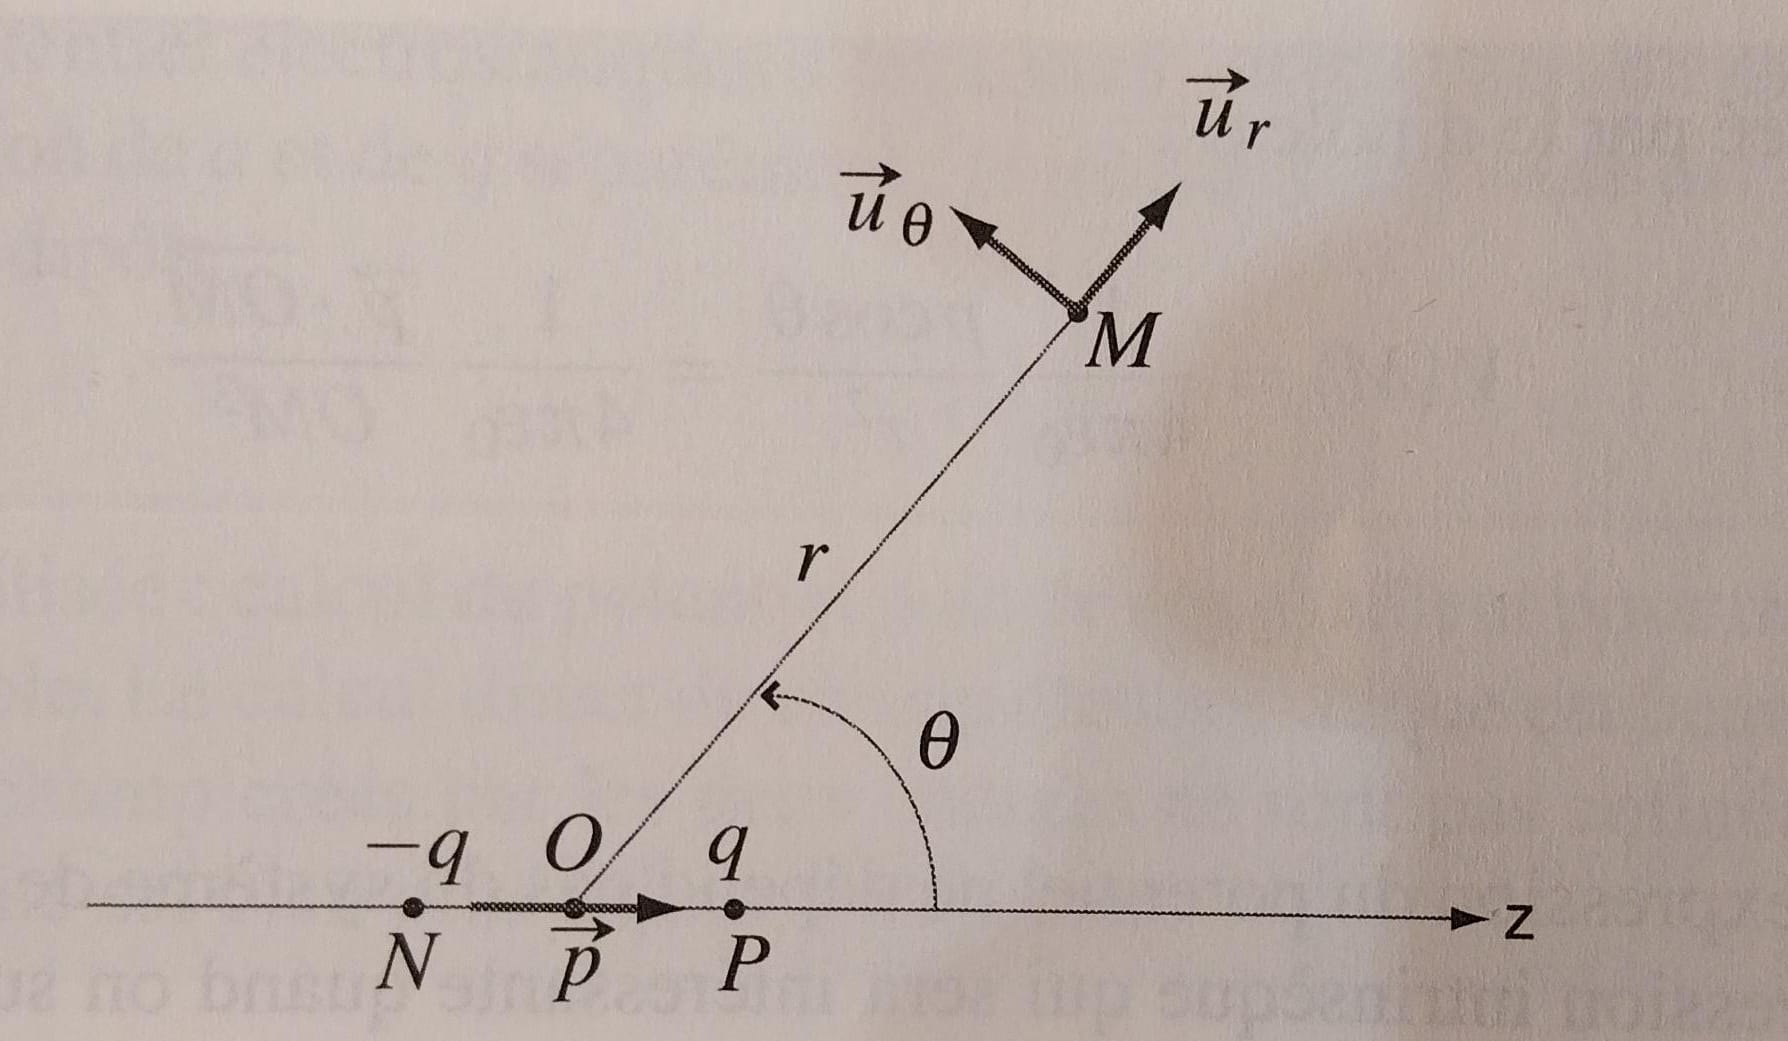
\includegraphics[width=0.4\textwidth]{dipôle schéma.jpg}
    \caption{Dipôle électrostatique}
\end{figure}

Le potentiel électrique créé par un dipôle en un point $M$ loin du dipôle vaut : \\
$$ V(M) = \dfrac{1}{4\pi \varepsilon_0} \dfrac{\vec{p}.\vec{OM}}{OM^3} $$


\textbf{Propriétés: }
\begin{enumerate}
  \item La résultante des forces subies par un dipôle dans un champ électrique uniforme est nulle.
  \item Dans un champ uniforme, le dipôle tend à s'aligner avec le champ.
  \item Dans un champ non unifome, la résultante des forces vaut $\vec{F} =(\vec{p}.\vec{grad})\vec{E}$. 
  \item Le moment des forces subi par un dipôle dans un champ électrique quelconque en un point $A$ est $\vec{M_A} = \vec{p} \wedge \vec{E(A)}$. 
  \item L'énergie potentielle d'un dipôle \textbf{rigide} situé en un point $A$ vaut $E_p = -\vec{p}.\vec{E(A)}$.
\end{enumerate}

\textbf{Polarisabilité: }
Lorsqu'un atome ou une molécule est soumise à un champ électrique $\vec{E}$, les charges qui la composent se déplacent et créent un dipôle induit $\vec{p_{ind}}$. On définit alors la polarisabilité $\alpha$ ainsi: 
$$ \vec{p_{ind}} = \alpha \epsilon_0 \vec{E} $$. 

\textbf{Capacités exigibles: }

\begin{itemize}
  \item Savoir calculer le potentiel créé par un dipôle et en déduire le champ (attention, pas l'inverse).
  \item Dessiner l'allure des lignes de champ et des lignes équipotentielles d'un dipôle. 
  \item Retrouver la résultante des forces et des moments subis par un dipôle dans un champ électrique uniforme et quelconque. 
  \item Connaître et retrouver l'énergie potentielle d'un dipôle plongé dans un champ $\vec{E}$. 
  \item Retrouver la polarisabilité de l'atome d'hydrogène dans le modèle de Thomson. 
\end{itemize}


\section{Potentiel de Yukawa} 
Soit $\rho(r)$ une distribution de charge à symétrie sphérique créant le potentiel $V(r) = \frac{q^*e^{-\frac{r}{a}}}{4 \pi \varepsilon_0 r }$.
\begin{enumerate}
    \item Déterminer le champ électrique dans tout l'espace et en donner un équivalent pour $r \rightarrow 0$. Que pense-t-on de la distribution de charge en 0 ? 
    \item En utilisant le théorème de Gauss, montrer que $\rho(r) = \varepsilon_0 \frac{1}{r^2} \frac{d}{dr}(r^2 E(r))$. En déduire $\rho(r)$. 
    \item Calculer la charge totale contenue dans une sphère de rayon $R$ centrée en 0.
    \item En déduire la charge au centre.
\end{enumerate}

\section{Modèle de Thomson}

\begin{itemize}
  \item Rappeler le modèle de Thomson.
  \item Calculer la polarisabilité de l'atome d'hydrogène dans ce modèle.
\end{itemize}

\section{Deux sphères de densité opposées}

On considère deux sphères de rayon $R$ de densité volumique de charge $\rho$ et $-\rho$ respectivement.
Les centres de ces deux sphères sont décalés de $a <<R$. 
\begin{enumerate}
  \item Déterminer le champ électrostatique dans la zone située à l'intérieur des deux sphères et à l'extérieur des deux sphères. 
  \item Montrer qu'on peut définir un moment dipolaire tel que le champ à l'extérieur des deux sphères soit égal au champ créé par un moment dipolaire. \\[2cm]
\end{enumerate}


% \begin{figure}[h]
%   \centering
%   
\includegraphics[width=0.4\textwidth]{meme.jpg}
% \end{figure}



\end{document}

